\chapter{Protecting Insecure Web Application}
\label{Protecting Insecure Web Application}
\section{Introduction}

The hands-on laboratory is mean to teach system administrator's how to protect insecure web application from common attacks like injection's, \gls{XSS}, \gls{CSRF}, brute force, file upload and file inclusion. Damn Vulnerable Web Application \gls{DVWA} is used as role of insecure application.


\subsection{Lab Scenario}
Lab participant acts as system administrator for small company which has several web applications. One legacy application is tremendously vulnerable for common type of attacks. Company ordered new web application to replace old and vulnerable service. However old application must survive at least few month's before being replaced. Till that time system administrator have high criticality task  to protect this vulnerable system. Blocking IP addresses is not a solution because client's requests can be originated from any location, although fixing all programming errors takes too long and new version of software was developed for that purposes.

\subsection{Final System Architecture} 
Keep in mind that final architecture contains several components to provide layered security for insecure web application as seen on Figure ~\ref{Architecture of Secured Web Application}

\begin{figure}[H] 
 \centering 
 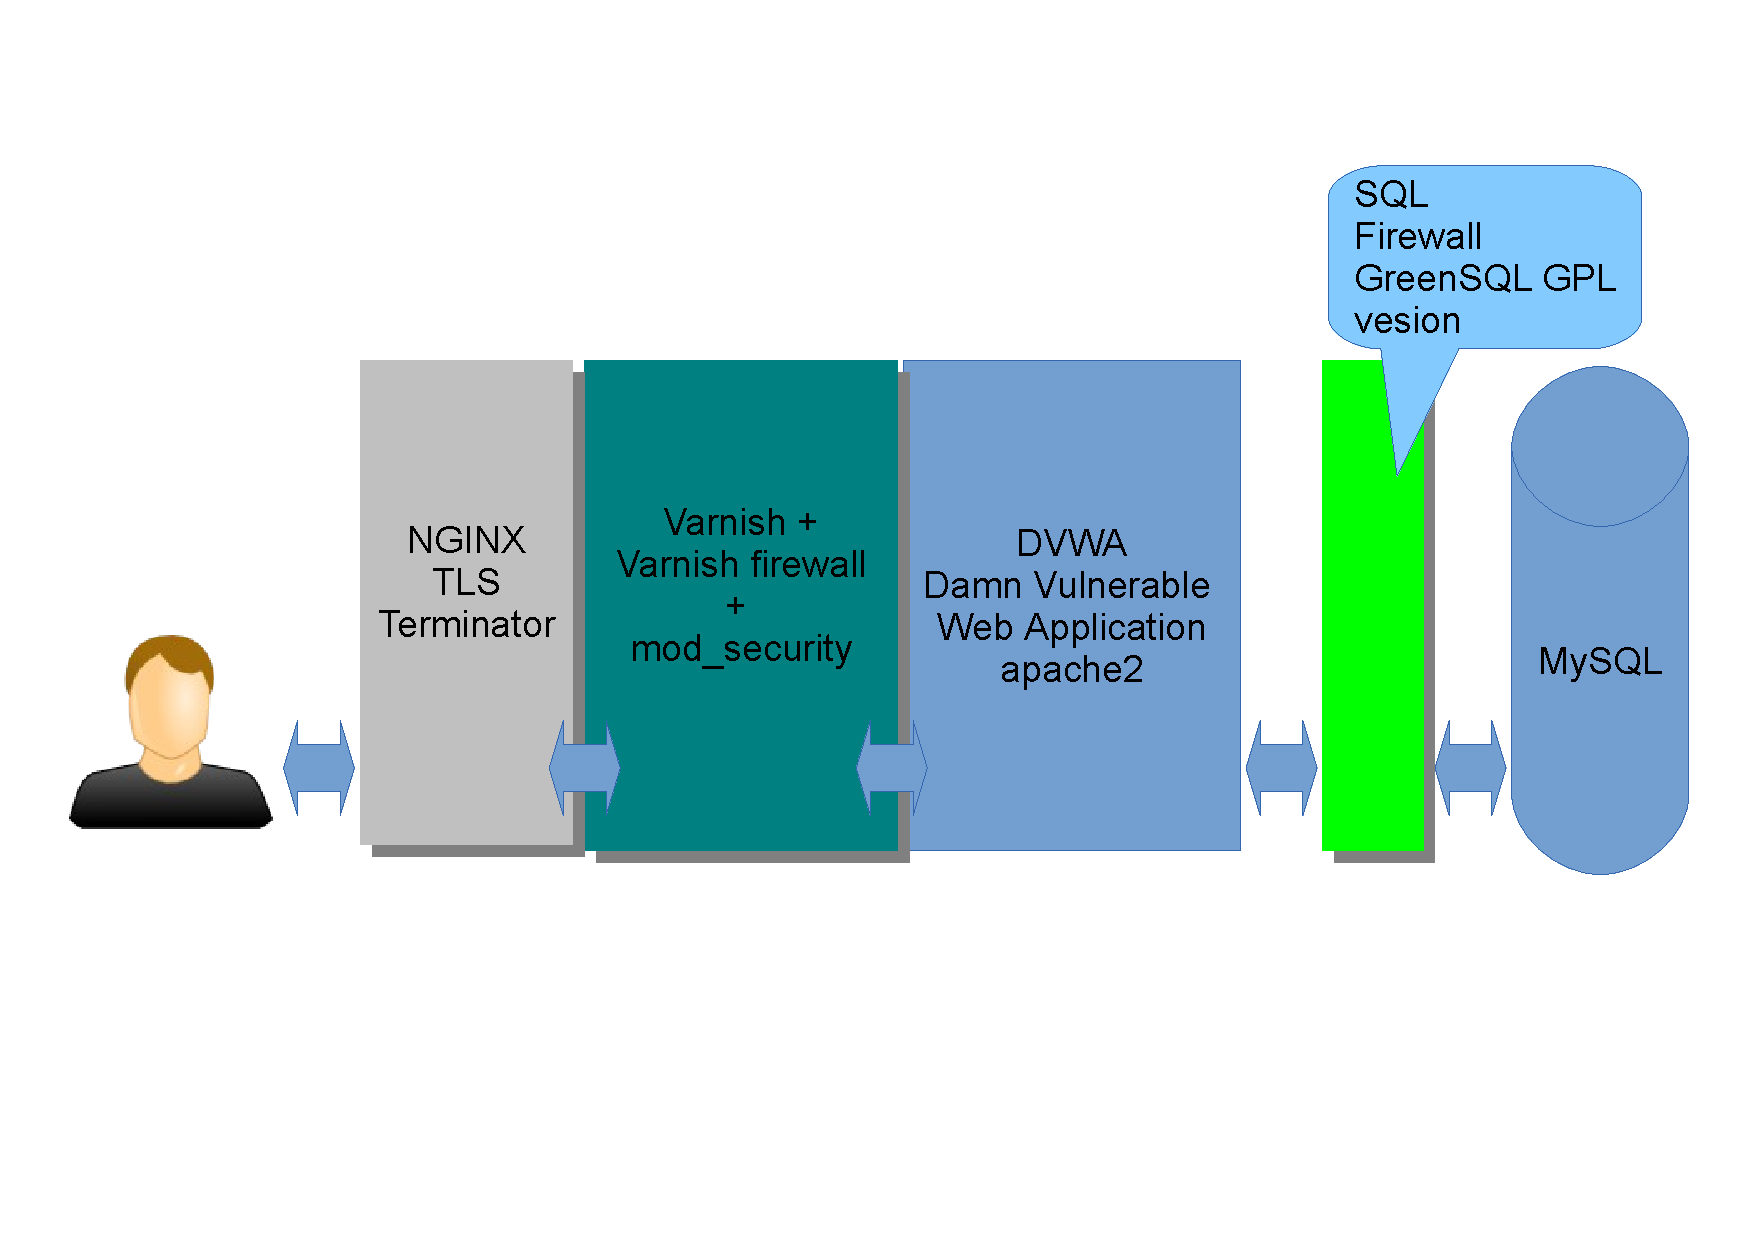
\includegraphics[width=0.9\textwidth]{web_security_lab_goal.pdf} 
 \caption{Architecture of Secured Web Application} 
 \label{Architecture of Secured Web Application} 
\end{figure}

%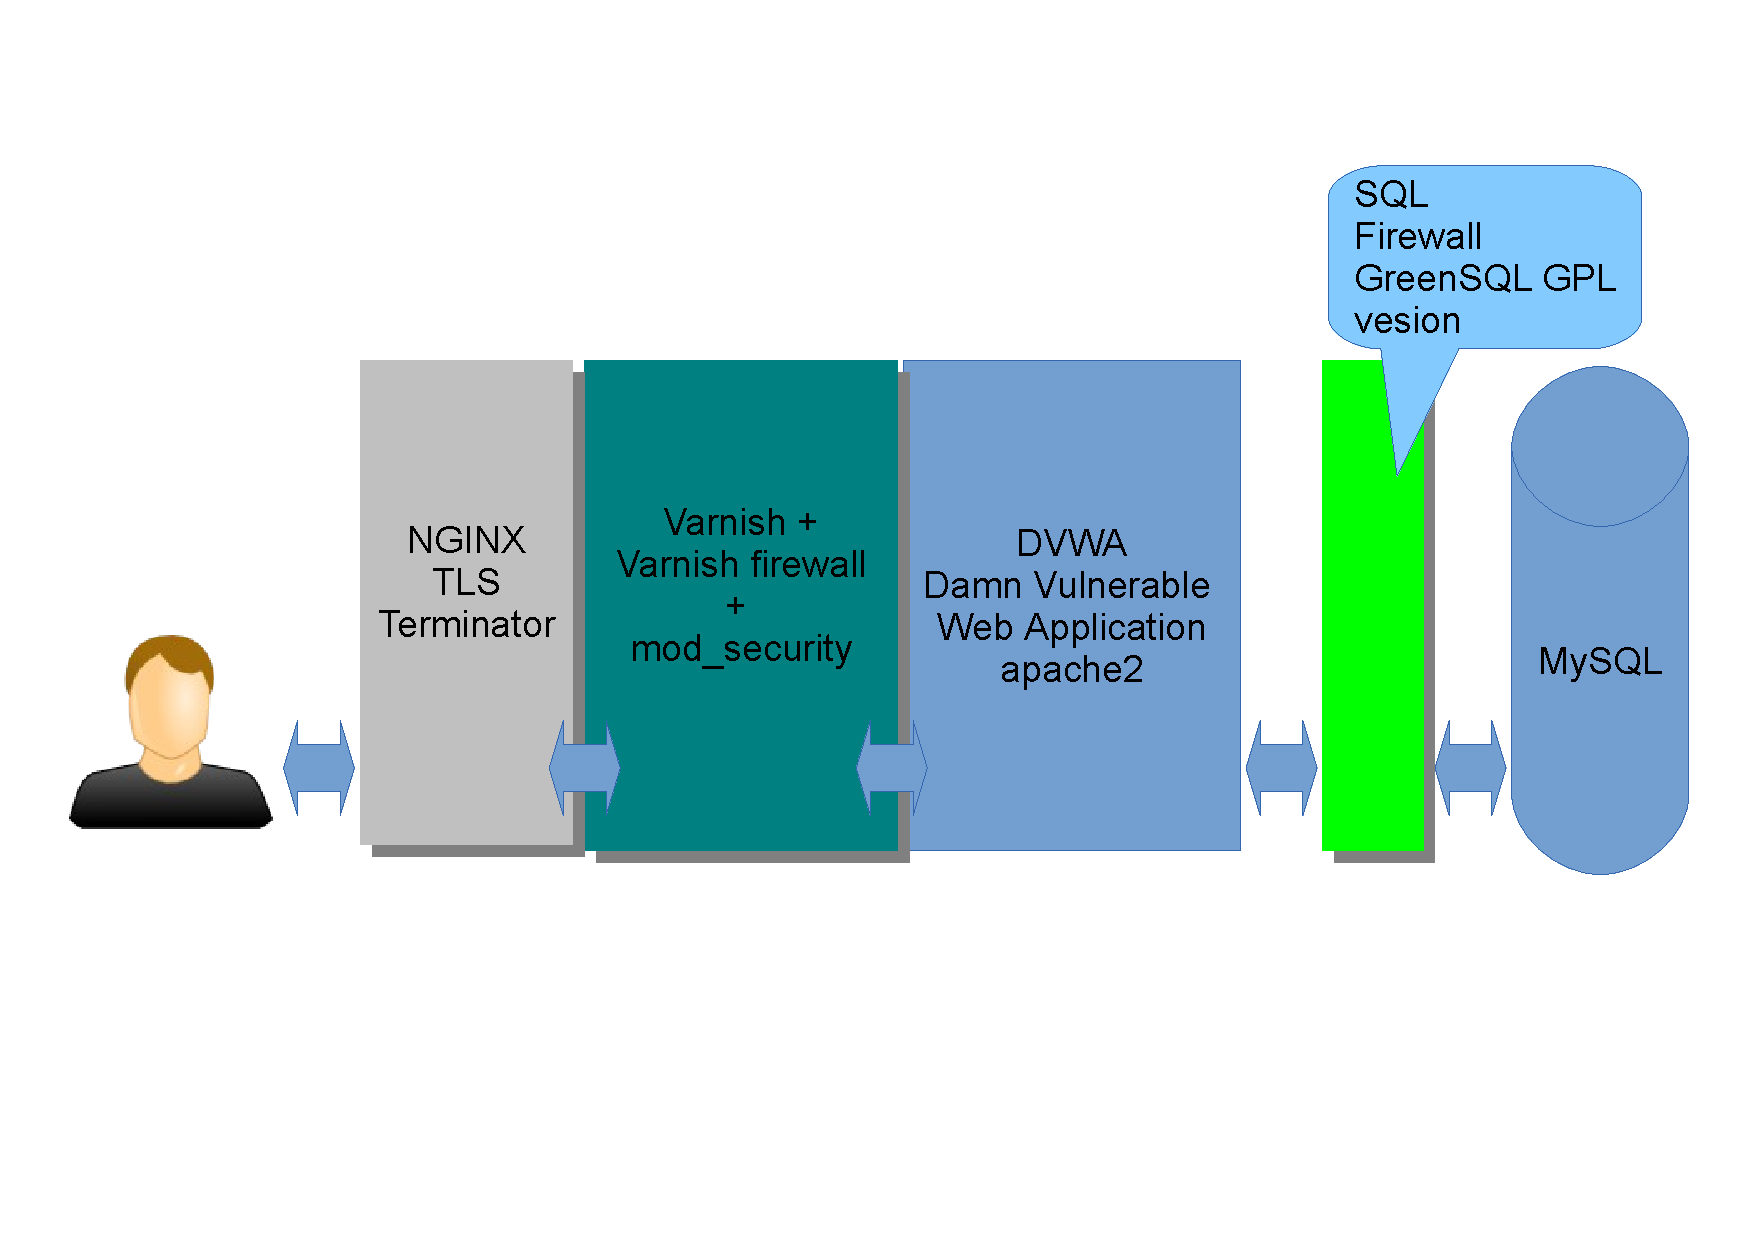
\includegraphics[width=\textwidth]{web_security_lab_goal.pdf}

\section{Pre-Requirements} 
\section{Scope}
\section{Learning Outcomes} 
\section{Setting up the Virtual Environment}
\section{Installation of Damn Vulnerable Web Application}
\subsection{Introduction to DVWA}

Ensure that you have administrator rights
\mint[frame=lines, framesep=1mm]{bash}|sudo -i|
Ensure that unzip package is installed
\begin{minted}[frame=lines,framesep=2mm]{bash}
type unzip || apt-get install unzip
\end{minted}
Dowload DVWA using web get utility wget
\mint[frame=lines, framesep=1mm]{bash}|wget http://dvwa.googlecode.com/files/DVWA-1.0.7.zip|

\begin{minted}[frame=lines,framesep=2mm]{bash}
unzip DVWA-1.0.7.zip
mv dvwa /var/www

nano /var/www/dvwa/config/config.inc.php

$_DVWA[ 'db_user' ] = 'root';
$_DVWA[ 'db_password' ] = 'student';
$_DVWA[ 'db_database' ] = 'dvwa';
\end{minted}
%$
For save use  CTRL + X


http://$ServerIP$/dvwa/
Username : admin
Password : password
Change DVWA Security level to low (for beginners)

\begin{figure}[H] 
 \centering 
 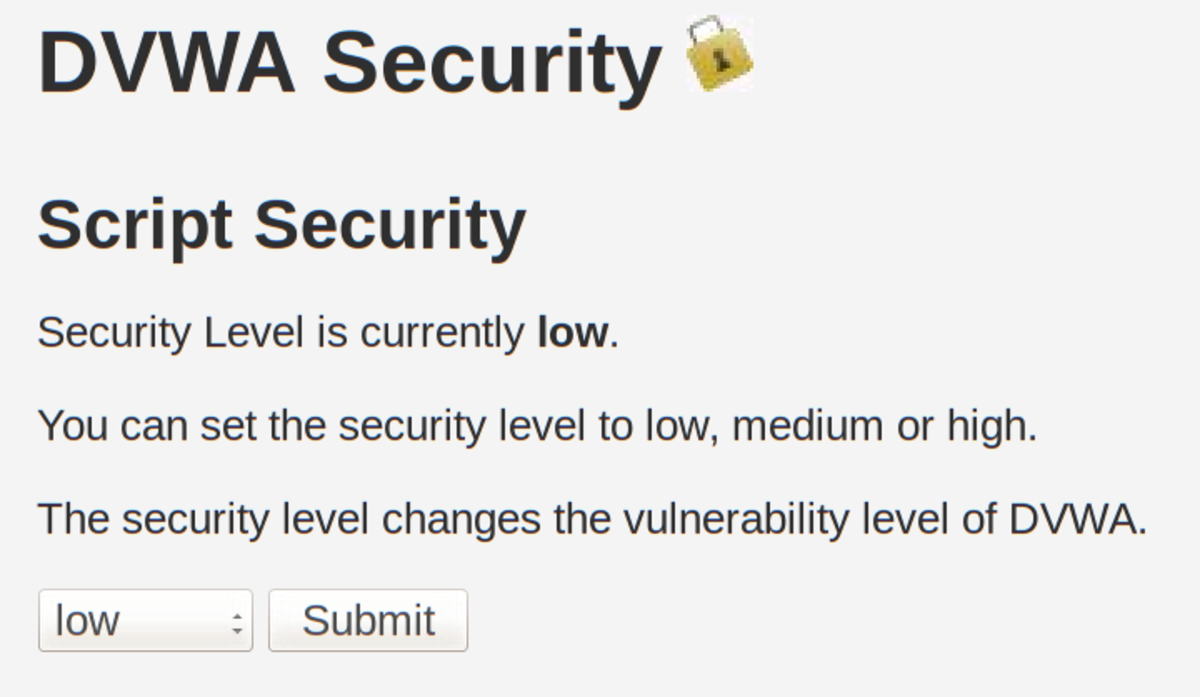
\includegraphics[width=0.6\textwidth]{dvwa_security_low.pdf} 
 \caption{Setting DVWA Security Level to Low} 
 \label{Setting DVWA Security Level to Low} 
\end{figure}


\begin{figure}[H] 
 \centering 
 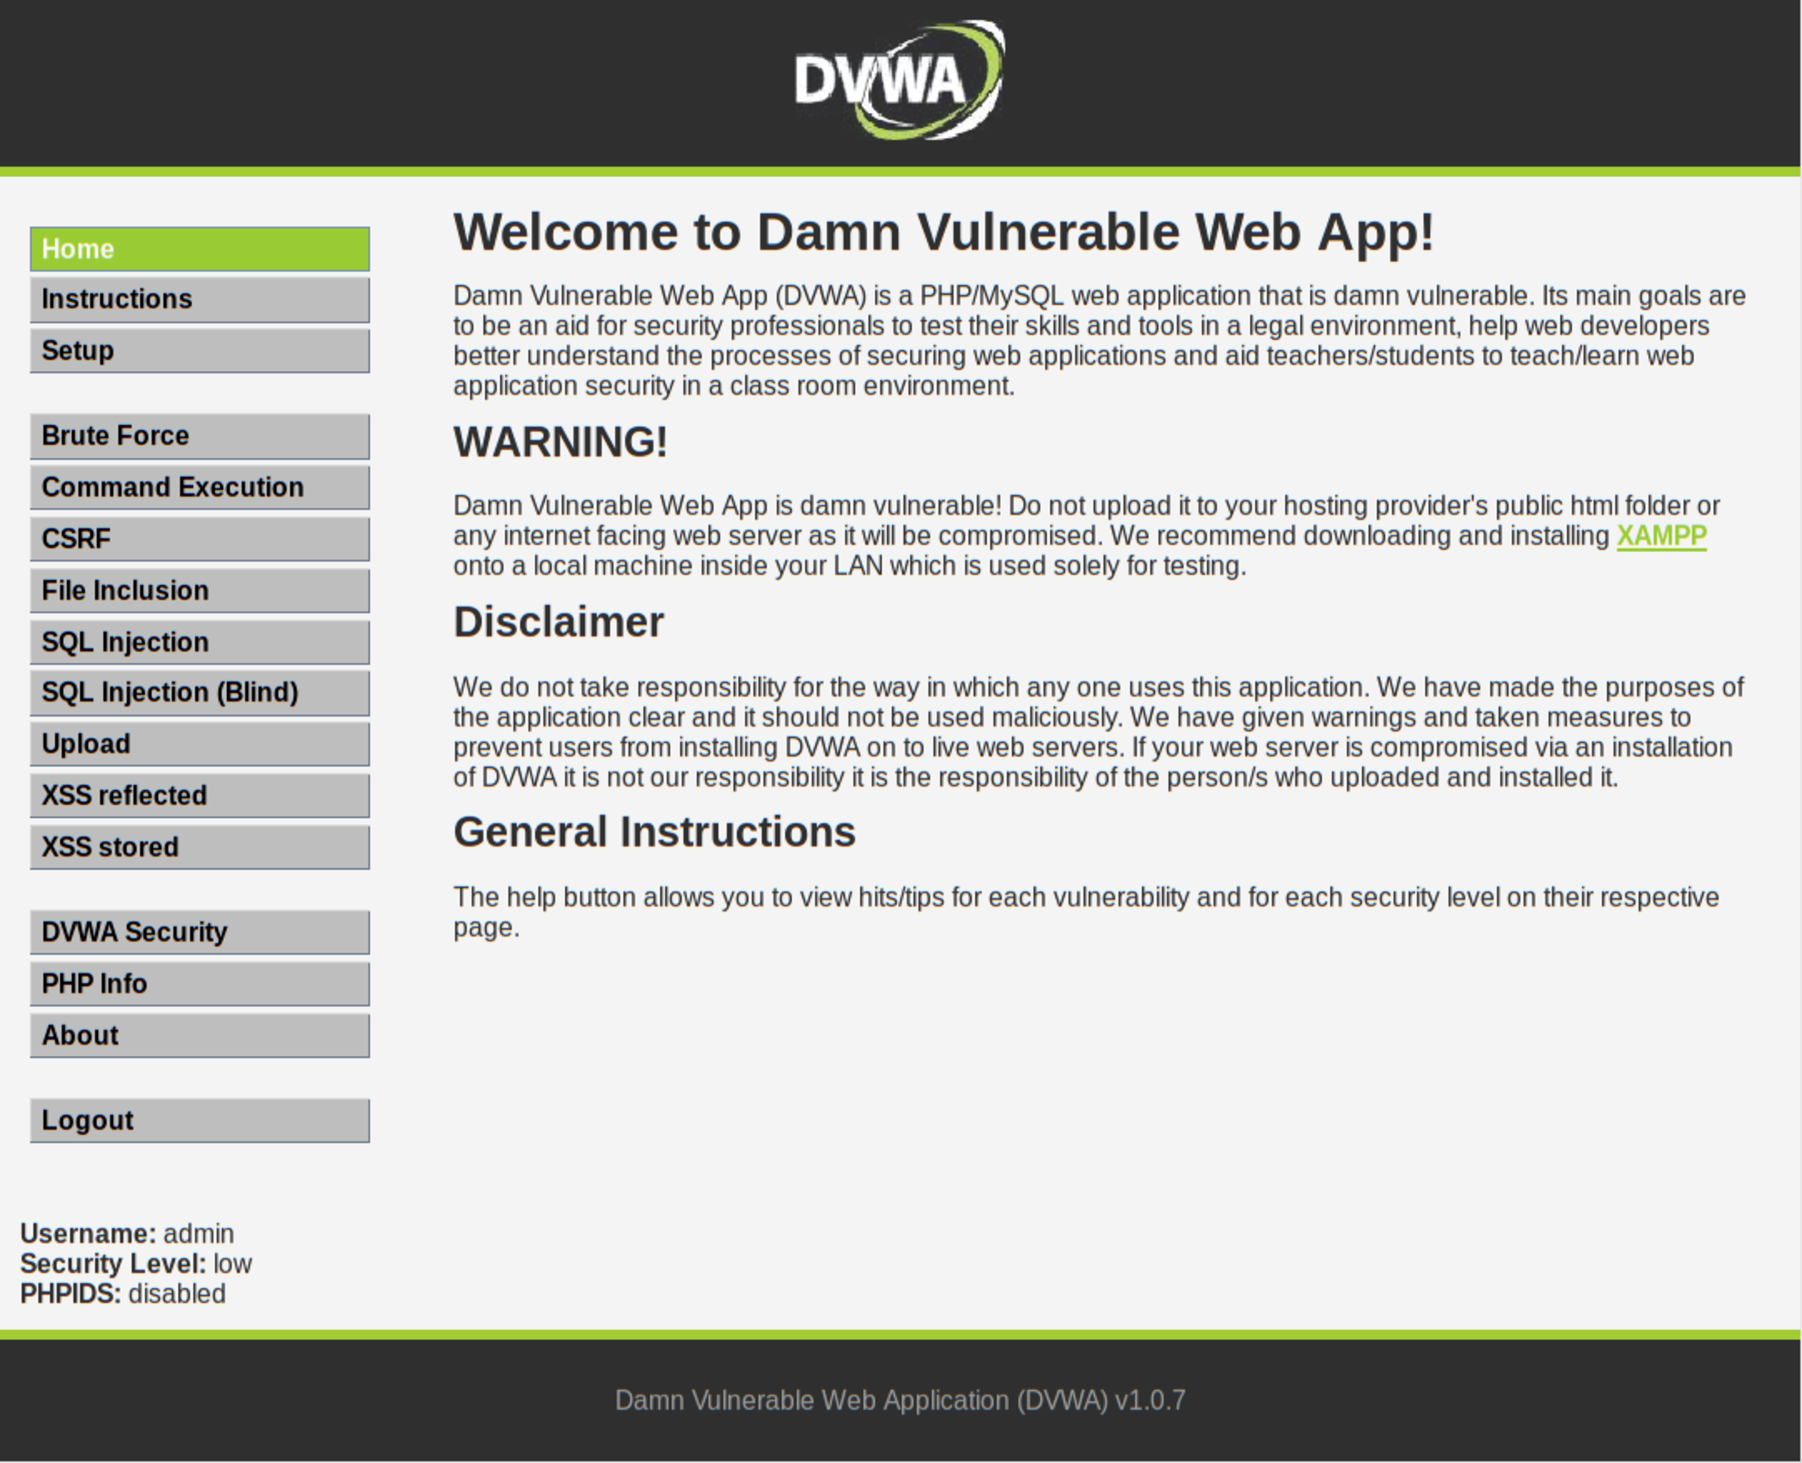
\includegraphics[width=0.8\textwidth]{DVWA_Main_Page.pdf} 
 \caption{Damn Vulnerable Web Application - Homepage} 
 \label{Damn Vulnerable Web Application - Homepage} 
\end{figure}
